\documentclass[11pt]{article}

\usepackage[margin=1in]{geometry}
\usepackage{amsmath, amssymb}
\usepackage{listings}
\usepackage{xcolor}
\usepackage{hyperref}
\usepackage{enumitem}
\usepackage{titlesec}
\usepackage{parskip}
\usepackage{booktabs}
\usepackage{tcolorbox}
\usepackage{tikz}
\usetikzlibrary{arrows.meta, positioning, shapes.geometric}

\lstset{
    basicstyle=\ttfamily\small,
    keywordstyle=\color{blue}\bfseries,
    commentstyle=\color{gray}\itshape,
    stringstyle=\color{red},
    frame=single,
    breaklines=true,
    showstringspaces=false,
    tabsize=4
}

\newtcolorbox{keyidea}[1][]{colback=blue!5, colframe=blue!50!black,
    fonttitle=\bfseries, title=Key Idea, #1}

\newtcolorbox{keytip}[1][]{colback=green!5, colframe=green!50!black,
    fonttitle=\bfseries, title=Tip, #1}

\newtcolorbox{keyintuition}[1][]{colback=orange!5, colframe=orange!50!black,
    fonttitle=\bfseries, title=Intuition, #1}

\title{\textbf{CS3210: Operating Systems} \\ Lecture 9 --- VMM Finale: Tips and Tricks}
\author{John Kim \\ Georgia Institute of Technology}
\date{February 12, 2026}

\begin{document}
\maketitle
\tableofcontents
\newpage

% ============================================================
\section{Introduction: The Full Toolkit of VM Tricks}
% ============================================================

Virtual memory management is one of the most powerful tools in an operating system's toolkit. By decoupling virtual addresses from physical memory, the OS gains the ability to implement a rich set of optimizations and features that would be impossible with bare physical addressing. This lecture covers the remaining tricks enabled by paging beyond the copy-on-write (CoW) fork mechanism discussed in Lectures 7--8.

The complete list of VM tricks includes the following:

\begin{enumerate}
    \item Copy-on-write fork — avoid copying data on fork; copy pages only when written.
    \item Demand paging or lazy allocation — avoid allocating physical memory until pages are actually accessed.
    \item On-demand zero-filled pages — defer zeroing of freshly allocated pages until access time.
    \item Single zero-filled page sharing — multiple virtual pages map to one read-only zero physical page.
    \item Virtual allocation — allocate virtual address space without reserving physical memory.
    \item Virtual shared memory — multiple processes share the same physical pages.
    \item Memory-mapped files — map file contents directly into virtual address space.
    \item Paging to disk (swap) — move physical pages to disk when memory is scarce.
    \item Memory oversubscription — commit more virtual memory than physical memory is available.
\end{enumerate}

Lectures 7 and 8 introduced copy-on-write fork in detail. This lecture completes the picture by exploring the remaining optimizations. Each trick exploits the fundamental property that the OS controls the page table and can intercept memory accesses via page faults. The recurring theme is \textbf{deferral}: instead of performing expensive operations eagerly (allocation, zeroing, copying), the OS performs them lazily, only when truly necessary.

% ============================================================
\section{Lazy Allocation and Demand Paging}
% ============================================================

When a process calls \texttt{sbrk()} to grow its heap, or when a new process is created via \texttt{fork()}, does the OS immediately allocate physical memory for all requested virtual pages? The answer is no. \textbf{Lazy allocation}, also called \textbf{demand paging}, defers physical allocation until the process actually accesses the page.

\subsection{The Motivation: Oversubscription}

Consider a fork-heavy workload. A parent process has a large heap, perhaps hundreds of megabytes. It forks a child, which then executes a different program via \texttt{exec()}. Allocating and copying all those pages eagerly is wasteful: the child will immediately discard its inherited address space and replace it with the new program's code and data. In a system with lazy allocation, the OS can assign virtual address space and mark pages as not present (P=0 in the page table) without allocating physical frames. The pages only become physically resident when accessed.

More broadly, lazy allocation enables \textbf{memory oversubscription}: the OS can commit more total virtual memory to processes than physical memory is actually available. As long as not all processes access their full virtual allocations simultaneously, the system thrives.

\subsection{Implementation}

When a process requests more virtual memory (via \texttt{sbrk()} or a malloc library call), the OS updates the process's internal state to record the new heap size (e.g., \texttt{myproc()->sz} in xv6) but does \emph{not} populate the page table. PTEs for the newly requested region remain invalid (P=0). When the process attempts to read or write a page in that region, the MMU raises a page fault. The OS handles the fault in the page fault handler:

\begin{enumerate}
    \item Check whether the faulting virtual address falls in a valid (allocated but not yet resident) region. This requires the OS to maintain allocation metadata separate from the page table.
    \item If valid, allocate a free physical frame.
    \item Initialize the frame (if needed; see lazy zeroing below).
    \item Insert a valid PTE into the page table pointing to the newly allocated frame.
    \item Return from the exception, and the instruction retries. This time the page is resident and the memory access succeeds.
\end{enumerate}

\subsection{Tradeoffs}

Lazy allocation introduces a tradeoff between initial cost and runtime cost:

\begin{center}
\begin{tabular}{lll}
\toprule
\textbf{Strategy} & \textbf{Allocation Cost} & \textbf{Runtime Behavior} \\
\midrule
Eager allocation & O(n) upfront & No page faults for allocated pages \\
Lazy allocation & O(1) per request & Page faults spread over execution \\
\bottomrule
\end{tabular}
\end{center}

Eager allocation guarantees that physical memory is reserved at allocation time. If the OS accepts the allocation, the process will never suffer an out-of-memory (OOM) error on access. Lazy allocation defers the cost but risks OOM exceptions if the system runs out of memory before all requested pages are accessed. This is acceptable in modern systems: the OS can then use the OOM killer to terminate lower-priority processes and free up memory.

\begin{keyidea}
Lazy allocation exploits the observation that processes often allocate more memory than they use. By deferring physical allocation to access time, the OS reduces fork() cost and enables memory oversubscription.
\end{keyidea}

% ============================================================
\section{Lazy Zeroing}
% ============================================================

Physical memory returned from the free list must be \textbf{zeroed} before being given to a process. If a page contains residual data from a previously freed page (which may have belonged to a different process), that data would leak to the new owner. This is a severe security vulnerability: an attacker could craft memory allocation patterns to capture sensitive data (cryptographic keys, passwords, private data) from other processes.

\subsection{Eager Zeroing}

A naive implementation zeros pages eagerly: when allocating a physical frame, the OS immediately executes \texttt{memset(frame, 0, PGSIZE)} before returning the page to the process. This is correct but expensive. Zeroing a full 4~KB page requires hundreds of CPU cycles and memory bus traffic.

\subsection{Lazy Zeroing: On-Access Zeroing}

Instead, the OS can defer zeroing until the page is accessed. Here is the strategy:

\begin{enumerate}
    \item When allocating a frame, insert a special PTE that marks the page as \emph{zero-on-use}. This PTE is invalid (P=0) but carries metadata (e.g., a special flag in the OS's PTE metadata structure) indicating it should be zeroed on first access.
    \item When the process accesses the page, a page fault fires.
    \item In the fault handler, the OS recognizes the zero-on-use marker, zeros the frame, and marks the PTE as valid (P=1).
    \item The instruction retries and succeeds.
\end{enumerate}

This trades the cost of a page fault (hundreds of cycles) against the cost of eager zeroing (hundreds of cycles). The benefit is that if the page is never accessed, the zeroing cost is avoided entirely.

\begin{keytip}
Lazy zeroing is most effective for pages that are allocated but never accessed---a common pattern in large memory allocations or initialization of sparse data structures.
\end{keytip}

% ============================================================
\section{Single Zero Page Optimization}
% ============================================================

Many newly allocated pages are zero-filled. In a system with thousands of processes, each holding multiple zero-filled pages, there could be millions of physical pages containing only zeros. This is wasteful: each page consumes memory, a TLB entry, and (potentially) page table memory.

The \textbf{single zero page optimization} is a clever technique to compress these redundant pages. Instead of allocating a separate physical page for each zero-filled virtual page, the OS maintains a single read-only physical zero page. All virtual pages that should be zero-filled are mapped to this one page.

\subsection{Basic Mechanism}

When the OS needs to provide a zero-filled page, instead of allocating a fresh physical frame and zeroing it, the page table entry points to the global zero page with the following properties:

\begin{itemize}
    \item The PTE marks the page as present (P=1) and valid.
    \item The PTE marks the page as \textbf{read-only} (W=0 in the permissions).
    \item All zero-filled virtual pages (across all processes, if desired) may point to this same physical page.
\end{itemize}

When the process reads from this page, it reads zeros. Correct and efficient. But what if the process tries to write to the page?

\subsection{Copy-on-Write for Zero Pages}

Writing to a read-only page triggers a protection fault---another form of page fault. The OS handles it as follows:

\begin{enumerate}
    \item Recognize that the fault is due to a write to the zero page.
    \item Allocate a fresh physical frame.
    \item Zero the new frame (or skip zeroing if the old page was already zeroed).
    \item Update the PTE to point to the new frame with write permission (W=1).
    \item Mark the old zero page's reference count unchanged (since many processes may still map to it).
    \item Return, and the instruction retries. The write now succeeds on the private page.
\end{enumerate}

This is \textbf{copy-on-write applied specifically to zero pages}. The pattern is identical to CoW fork: share until written, then copy.

\begin{keyintuition}
The zero page is the ultimate sharing scenario: if a page contains only zeros, why allocate a unique physical frame for every virtual page that needs zeros? Share one read-only zero page and copy on write.
\end{keyintuition}

\subsection{Example: Virtual Address Space Growth}

Consider a process in xv6 with three allocated heap pages (P1, P2, P3), each mapped to physical pages F1, F2, F3, with write permission. The process's memory size is tracked in \texttt{myproc()->sz} = 3 PGSIZE. The process calls \texttt{sbrk(2*PGSIZE)} to grow its heap by two pages.

\begin{enumerate}
    \item The OS updates \texttt{myproc()->sz} to 5 PGSIZE (lazy allocation).
    \item Virtual pages P4 and P5 are assigned, but their PTEs are not immediately valid.
    \item When the process first accesses P4 or P5, a page fault fires.
    \item The fault handler allocates a physical frame and initializes it. To save cost, instead of allocating two separate frames, both P4 and P5 are mapped to the global read-only zero page.
    \item When the process writes to P4, a protection fault occurs. The OS allocates a new frame F4, zeros it (or reuses the zero content), updates P4's PTE to point to F4 with write permission (W=1), and the write succeeds.
    \item P5 remains mapped to the global zero page until the process writes to it.
\end{enumerate}

This reduces the number of allocated physical frames and avoids redundant zeroing.

\subsection{TikZ Diagram: Single Zero Page Optimization}

\begin{figure}[h]
\centering
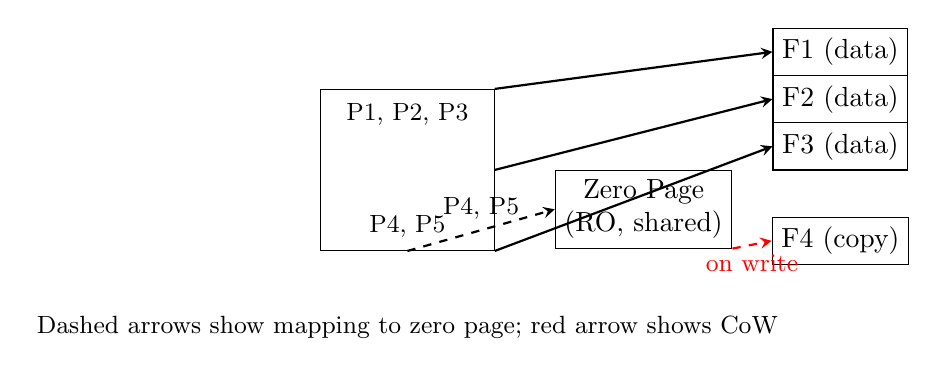
\begin{tikzpicture}[
    node distance=1.2cm,
    box/.style={rectangle, draw, minimum width=1.5cm, minimum height=0.6cm},
    bigbox/.style={rectangle, draw, minimum width=1.5cm, minimum height=1.8cm},
    arrow/.style={->, >=stealth, thick},
    label/.style={font=\small}
]

% Virtual Address Space (left)
\node[bigbox, label=left:{Virtual AS}] (virt) at (0, 0) {
    \begin{tabular}{c}
        P1, P2, P3 \\
        \\ [2em]
        P4, P5
    \end{tabular}
};

% Zero Page (center)
\node[box, align=center] (zeropage) at (3, -0.5) {Zero Page \\ (RO, shared)};

% Physical Pages (right)
\node[box] (F1) at (5.5, 1.5) {F1 (data)};
\node[box] (F2) at (5.5, 0.9) {F2 (data)};
\node[box] (F3) at (5.5, 0.3) {F3 (data)};
\node[box] (F4) at (5.5, -0.9) {F4 (copy)};

% Arrows from virtual to physical
\draw[arrow] (virt.north east) -- (F1.west);
\draw[arrow] (virt.east) -- (F2.west);
\draw[arrow] (virt.south east) -- (F3.west);
\draw[arrow, dashed] (virt.south) -- (zeropage.west) node[midway, above, label] {P4, P5};

% Arrow from zero page to F4 (after CoW)
\draw[arrow, dashed, red] (zeropage.south east) -- (F4.west) node[midway, below, label, red] {on write};

% Legend
\node[label] at (0, -2) {\small Dashed arrows show mapping to zero page; red arrow shows CoW};

\end{tikzpicture}
\caption{Single Zero Page Optimization: Multiple virtual pages (P4, P5) initially map to a shared read-only zero page. On write to P4, a new physical frame F4 is allocated (copy-on-write).}
\end{figure}

% ============================================================
\section{Shared Memory}
% ============================================================

Virtual memory decouples addresses from physical frames, enabling multiple virtual addresses to map to the same physical page. This is the basis of \textbf{shared memory}: two or more processes can have entries in their respective page tables that point to the same physical frame.

\subsection{Motivation and Use Cases}

Shared memory is powerful for high-performance scenarios:

\begin{itemize}
    \item \textbf{Shared libraries}: libc, libm, libpthread, and other standard libraries are loaded once into physical memory. Every process that uses them maps the same physical pages into its virtual address space. Code sharing (read-only text segments) is universal. Data segments may use copy-on-write.
    \item \textbf{Distributed computing}: in high-performance computing (HPC) clusters, multiple processes running on the same node may need to communicate efficiently. Rather than copying data through the kernel, shared memory allows processes to access a common buffer directly.
    \item \textbf{Inter-process communication (IPC)}: POSIX shared memory (shm\_open, mmap) and SysV shared memory (shmget, shmat) allow processes to create anonymous shared regions for fast data exchange.
\end{itemize}

\subsection{Implementation}

Creating a shared memory region requires OS support. In modern Unix systems:

\begin{enumerate}
    \item A process or the kernel establishes a physical memory region (allocated but not yet mapped to any virtual address).
    \item Process A inserts a PTE into its page table pointing to this region, with appropriate permissions (read, write).
    \item Process B inserts a PTE into its page table pointing to the \emph{same physical frames}.
    \item Both processes can now read and write the shared region. Writes by one process are immediately visible to the other.
\end{enumerate}

If the region is large or frequently modified, the OS must ensure cache coherency: updates to shared memory must be visible across processes. Modern multicore CPUs provide hardware cache coherency, but this is worth verifying.

\subsection{Shared Libraries on Linux}

The \texttt{/proc/PID/maps} file shows the virtual memory layout of a process. Shared libraries appear as memory-mapped regions. For example:

\begin{lstlisting}[caption={Example /proc/self/maps output showing shared libraries}]
7ffff7dd5000-7ffff7dfd000 r-xp 00000000 08:03 12345678 /lib64/libc.so.6
7ffff7dfd000-7ffff7ffd000 ---p 00028000 08:03 12345678 /lib64/libc.so.6
7ffff7ffd000-7ffff8001000 r--p 00028000 08:03 12345678 /lib64/libc.so.6
7ffff8001000-7ffff8003000 rw-p 0002c000 08:03 12345678 /lib64/libc.so.6
\end{lstlisting}

The first region (r-xp) is the read-execute text segment of libc. It is shared across all processes using libc, reducing physical memory consumption. The subsequent regions show read-only (r--p) and read-write (rw-p) portions. The data segment (rw-p) may be CoW: each process initially shares the same physical data pages, but writes trigger page faults and private copies.

\begin{keyidea}
Shared memory allows multiple processes to map the same physical pages, enabling efficient library sharing, IPC, and distributed computing without data copying.
\end{keyidea}

% ============================================================
\section{Memory-Mapped Files}
% ============================================================

File I/O is traditionally performed via system calls: \texttt{read()} and \texttt{write()}. These calls involve copying data from disk to kernel buffers and then to user buffers (or vice versa). For large files or high-throughput workloads, these copies are expensive.

\textbf{Memory-mapped files} offer an alternative: the OS maps a file's contents directly into the process's virtual address space. Reads and writes to the mapped region access the file without explicit I/O system calls.

\subsection{Mechanism}

The POSIX \texttt{mmap()} system call establishes the mapping:

\begin{lstlisting}[language=C, caption={Memory-mapped file example}]
int fd = open("data.bin", O_RDONLY);
char *addr = mmap(NULL, file_size, PROT_READ,
                   MAP_SHARED, fd, 0);
// addr[0..file_size-1] contains file contents
char byte = addr[100];  // read from file
munmap(addr, file_size);
close(fd);
\end{lstlisting}

Internally, the OS performs the following:

\begin{enumerate}
    \item Allocate a virtual address range of size \texttt{file\_size}.
    \item Insert PTEs for this range, marking them as invalid (P=0) but recording metadata that they are backed by the file at offset 0.
    \item The file region may also be recorded in a file-backed page cache structure.
    \item When the process accesses a page in the mapped region, a page fault fires.
    \item The fault handler recognizes the page as file-backed and reads the appropriate block from disk into a physical frame (if not already cached).
    \item The PTE is updated to point to the frame, and the access retries.
\end{enumerate}

This is \textbf{demand paging applied to files}: pages are loaded on demand, and the OS page cache ensures that frequently accessed pages remain in memory.

\subsection{Advantages over read()/write()}

\begin{itemize}
    \item \textbf{No explicit copying}: the mapped region is the file. No intermediate kernel buffer.
    \item \textbf{Random access}: memory-mapped access is random (can jump to any byte), whereas read() is sequential.
    \item \textbf{Page cache efficiency}: the kernel manages which pages are resident, using LRU eviction if memory pressure rises.
    \item \textbf{Sparse files}: if a file is sparse (many holes), only accessed pages consume physical memory.
\end{itemize}

\subsection{Flags: MAP\_SHARED vs MAP\_PRIVATE}

The \texttt{MAP\_SHARED} flag indicates that writes to the mapped region immediately update the file. This is safe for read-only access or when multiple writers are coordinated. The \texttt{MAP\_PRIVATE} flag applies copy-on-write semantics: writes create private copies of modified pages in memory, and the original file is not updated. This is useful for scenarios like debuggers or language runtimes that want to inspect a binary without modifying it.

\subsection{TikZ Diagram: Memory-Mapped File Access}

\begin{figure}[h]
\centering
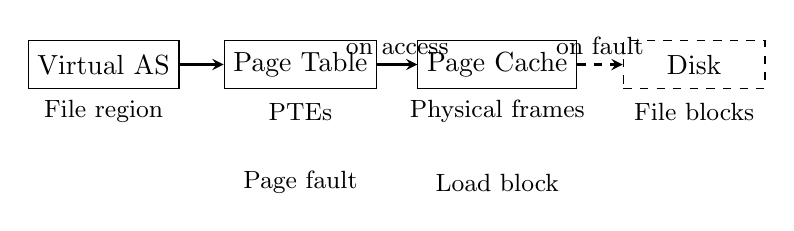
\begin{tikzpicture}[
    node distance=1.2cm,
    box/.style={rectangle, draw, minimum width=1.8cm, minimum height=0.6cm},
    diskbox/.style={rectangle, draw, dashed, minimum width=1.8cm, minimum height=0.6cm},
    arrow/.style={->, >=stealth, thick},
    label/.style={font=\small}
]

% Virtual Address Space
\node[box] (virt) at (0, 1.5) {Virtual AS};
\node[label] (v1) at (0, 0.9) {File region};

% Page Table
\node[box] (pt) at (2.5, 1.5) {Page Table};
\node[label] (pt1) at (2.5, 0.9) {PTEs};

% Page Cache (Physical Memory)
\node[box] (cache) at (5, 1.5) {Page Cache};
\node[label] (c1) at (5, 0.9) {Physical frames};

% Disk
\node[diskbox] (disk) at (7.5, 1.5) {Disk};
\node[label] (d1) at (7.5, 0.9) {File blocks};

% Page Fault Path
\node[label] (fault) at (2.5, 0) {Page fault};
\node[label] (load) at (5, 0) {Load block};

% Arrows
\draw[arrow] (virt) -- (pt);
\draw[arrow] (pt) -- (cache) node[midway, above, label] {on access};
\draw[arrow, dashed] (cache) -- (disk) node[midway, above, label] {on fault};

\end{tikzpicture}
\caption{Memory-Mapped File Access: Virtual pages map to a page cache backed by disk blocks. On page fault, the OS reads the corresponding block from disk into memory.}
\end{figure}

% ============================================================
\section{Memory Backing and Swap}
% ============================================================

Physical memory is finite. If all processes access their full virtual allocations simultaneously, the system runs out of memory. The OS addresses this via two mechanisms: \textbf{swapping} (or paging to disk) and \textbf{memory-backed pages}.

\subsection{Swapping and Page Replacement}

When physical memory is scarce, the OS can \textbf{evict} a physical page to disk, freeing the frame for other use. The evicted page is written to a designated swap area (a partition or file on disk). The page table entry for that virtual page is updated: P=0 (not present) and a secondary field stores the swap location (e.g., swap file offset).

When the process later accesses the evicted page, a page fault fires. The fault handler reads the page back from swap into a physical frame, updates the PTE, and the access retries. The OS uses a page replacement algorithm (e.g., LRU, clock algorithm) to choose which page to evict.

The cost of swapping is high: disk I/O is orders of magnitude slower than memory access. Modern systems try to minimize swapping by using memory caches, compression, and careful workload management. But swapping ensures that the system remains functional even under memory pressure.

\subsection{File-Backed Pages}

Pages mapped from files have a natural backing store: the file on disk. If the page is clean (unmodified), the OS can simply discard it and reload from the file later. This is much cheaper than writing to swap. The page cache maintains a \emph{dirty bit} to track which file-backed pages have been modified. Clean pages are evicted first; dirty pages are written to their backing file before eviction.

\subsection{Virtual Allocation and Oversubscription}

The combination of lazy allocation, swapping, and file-backed pages enables \textbf{memory oversubscription}: the OS can commit more virtual memory to processes than physical memory exists. As long as the total working set of all processes (the pages actively used at any moment) fits in physical memory, the system thrives. If the working set exceeds physical memory, the system enters a state of \textbf{thrashing}: pages are constantly evicted and reloaded, causing severe performance degradation. Modern OSs use swap accounting, cgroup memory limits, and the OOM killer to prevent or mitigate thrashing.

\begin{keytip}
Swapping allows the OS to provide more virtual memory than physical memory, but the cost is high. Design applications to minimize swap usage by respecting memory limits and managing memory carefully.
\end{keytip}

% ============================================================
\section{Linux Memory Introspection Tools}
% ============================================================

Understanding memory usage and allocation is crucial for system administration and application optimization. Linux provides several tools for inspecting memory:

\subsection{/proc/iomem}

The \texttt{/proc/iomem} file shows the physical memory layout:

\begin{lstlisting}[caption={Example /proc/iomem output}]
00000000-00000fff : Reserved
00001000-0009efff : System RAM
0009f000-0009ffff : Reserved
000f0000-000fffff : System ROM
00100000-dffeffff : System RAM
...
\end{lstlisting}

This reveals which physical memory regions are available for allocation, which are reserved for the kernel or devices, and which are ROM.

\subsection{/proc/self/maps and /proc/PID/maps}

The \texttt{maps} file shows the virtual memory layout of a process:

\begin{lstlisting}[caption={Example /proc/self/maps output}]
55555555b000-55555555c000 r--p 00000000 08:03 1234567 /bin/cat
55555555c000-555555561000 r-xp 00001000 08:03 1234567 /bin/cat
555555761000-555555763000 rw-p 00006000 08:03 1234567 /bin/cat
555555763000-555555784000 rw-p 00000000 00:00 0       [heap]
7ffff7dd5000-7ffff7dfd000 r-xp 00000000 08:03 1234568 /lib64/libc.so.6
7ffffffde000-7ffffffff000 rw-p 00000000 00:00 0       [stack]
\end{lstlisting}

Each line shows: virtual address range, permissions (r/w/x, p for private or s for shared), offset in the backing file, device number, inode, and pathname. This allows inspection of all mapped regions, including heap, stack, libraries, and memory-mapped files.

\subsection{pmap, free, and strace}

\begin{itemize}
    \item \texttt{pmap PID}: shows a more human-readable version of the memory map.
    \item \texttt{free}: displays system-wide memory usage (total, used, free, buffers, cache).
    \item \texttt{strace -e mmap,brk,mprotect PID}: traces memory-related system calls, useful for understanding allocation and protection changes.
\end{itemize}

% ============================================================
\section{Research Perspective: On-Demand Fork}
% ============================================================

Fork is a fundamental operation, but it has a hidden cost: even with copy-on-write, the OS must copy the page tables themselves. In modern applications with large address spaces (gigabytes), the page table can be enormous. Copying the page table at fork time is expensive.

\subsection{The Problem}

A process with 1 GB of allocated virtual memory has roughly $2^{30} / 2^{12} = 2^{18} \approx 262k$ page table entries. A fork() that copies the page table must perform 262k operations (or more, depending on the page table structure). On modern systems, page tables are hierarchical (e.g., 4-level paging on x86-64), so the cost grows with the tree structure.

In a system with many fork() calls (e.g., a web server forking workers, or a shell spawning commands), the fork() time dominates and becomes a bottleneck.

\subsection{On-Demand-Fork Solution}

The \textbf{On-Demand-Fork} technique (EuroSys 2021) extends copy-on-write to the page tables themselves: \textbf{page table page copy-on-write (PTP CoW)}. Instead of copying the entire page table on fork, the child initially shares the parent's page table pages (the intermediate levels of the page table tree). When the child (or parent) modifies a page table entry---adding, removing, or changing a mapping---a page table page fault fires, and the OS allocates a private copy of that page table page.

\subsection{Performance Results}

With 1 GB allocated memory:

\begin{itemize}
    \item \textbf{Traditional fork()}: 65x faster with PTP CoW.
    \item \textbf{Macro benchmarks}: 59--226\% execution throughput improvement in real-world applications (web servers, databases).
    \item \textbf{Micro benchmarks}: 99\% reduction in fork() invocation time.
\end{itemize}

The key insight is that for many workloads, the child process immediately execs a new program, so the shared page table pages are never modified. PTP CoW eliminates the unnecessary work.

\subsection{Limitations and Trade-offs}

PTP CoW adds complexity to the OS (new page fault types, page table page management). It also introduces latency spikes when a page table page is first modified (the fault handler must allocate, copy, and install the new PTE). But for fork-heavy workloads, the benefits far outweigh the costs.

\begin{keyidea}
On-Demand-Fork extends copy-on-write to page tables themselves, reducing fork() cost by 50--200x in large-address-space workloads by deferring page table copying until actually necessary.
\end{keyidea}

% ============================================================
\section{Research Perspective: Rapid VM Cloning}
% ============================================================

Virtual machine (VM) technology is fundamental to cloud computing. Cloning VMs---creating copies of a VM's full memory and disk state---is essential for rapid provisioning and elasticity. However, a VM with gigabytes of memory cannot be cloned instantly.

\subsection{Snowflock: Sub-Second VM Cloning}

\textbf{Snowflock} (EuroSys 2009, awarded the Test of Time Award at EuroSys 2023 for impact) applies demand paging and CoW to VM cloning. The key ideas:

\begin{enumerate}
    \item When the administrator requests a new VM clone, the hypervisor immediately forks the parent VM's memory image, but uses lazy CoW: both the parent and child VMs' memory regions share the same underlying physical pages.
    \item As one of the clones modifies memory pages, page faults trigger, and the OS allocates private copies. Multiple physical pages diverge from a common origin.
    \item Simultaneously, the system performs \emph{selective page transfer}: a background process identifies which pages the child VM is likely to access soon and pre-fetches them from the parent VM over the network, before the child accesses them. This hides the latency of page faults.
    \item The result: cloning a large VM in under one second, with negligible I/O overhead.
\end{enumerate}

This technology enabled rapid cloud VM provisioning, turning minutes of cloning time into seconds.

\subsection{Kaleidoscope: Stateful VM Replication at Scale}

\textbf{Kaleidoscope} (EuroSys 2011) extends rapid VM cloning with \textbf{state coloring}: tracking which pages in a VM contain which categories of state (e.g., application state, OS state, cold data). This enables \emph{selective replication}: instead of copying the entire VM, only the pages likely to be accessed in the clone are replicated initially. Cold pages are replicated on demand. This reduces both replication time and memory overhead, enabling cost-effective stateful VM replication in public clouds.

\subsection{Broader Implications}

These research systems demonstrate that the VM tricks discussed in this lecture---demand paging, CoW, shared memory, lazy allocation---are not just academic curiosities. They are the foundation of modern cloud infrastructure, enabling rapid provisioning, resource efficiency, and elasticity.

% ============================================================
\section{Summary}
% ============================================================

\begin{itemize}
    \item \textbf{Lazy allocation}: deferring physical memory allocation until page access reduces fork() cost and enables memory oversubscription.
    \item \textbf{Lazy zeroing}: deferring page zeroing until access time saves CPU cycles for pages that are never accessed.
    \item \textbf{Single zero page}: sharing one read-only zero-filled page across many virtual addresses, using CoW to create private copies on write.
    \item \textbf{Shared memory}: multiple processes map the same physical frames, enabling efficient library sharing, IPC, and distributed computing.
    \item \textbf{Memory-mapped files}: mapping file contents into virtual address space enables zero-copy file access and leverages the OS page cache.
    \item \textbf{Paging and swap}: evicting pages to disk enables memory oversubscription, though at high performance cost.
    \item \textbf{On-Demand-Fork}: extending CoW to page tables themselves reduces fork() cost by 50--200x in large-address-space systems.
    \item \textbf{Rapid VM cloning}: demand paging, CoW, and selective page transfer enable cloud VMs to be cloned in under a second, transforming cloud provisioning.
\end{itemize}

% ============================================================
\section{References}
% ============================================================

\begin{itemize}
    \item Intel Corporation. \textit{Intel 64 and IA-32 Architectures Software Developer's Manual}. 2023.
    \item Remzi Arpaci-Dusseau and Andrea Arpaci-Dusseau. \textit{Operating Systems: Three Easy Pieces}. Arpaci-Dusseau Books, 2015. \url{https://pages.cs.wisc.edu/~remzi/OSTEP/}
    \item Stephen D. Bonidie et al. ``\textit{Efficient and Scalable Paravirtual I/O}.'' USENIX ATC 2008.
    \item Yubin Ruan et al. ``\textit{On-Demand-Fork: A Fast Fork for Large Memory Workloads}.'' EuroSys 2021.
    \item Eno Thereska et al. ``\textit{Snowflock: Rapid Virtual Machine Cloning for Cloud Computing}.'' EuroSys 2009. (Test of Time Award EuroSys 2023)
    \item Wencong Xiao et al. ``\textit{Kaleidoscope: Cloud Micro-Elasticity via VM State Coloring}.'' EuroSys 2011.
    \item University of Washington. ``\textit{CSE 451: Operating Systems}.'' Lecture materials. \url{https://courses.cs.washington.edu/courses/cse451/}
    \item MIT. ``\textit{6.828: Operating System Engineering}.'' Lecture materials and xv6 kernel. \url{https://pdos.csail.mit.edu/6.828/}
\end{itemize}

% ============================================================
\section*{Personal Notes}
% ============================================================
% Add your own notes below this line

\end{document}
